\section{Simulation}
 \includeref{Phase is not localcised, due to infinite cosine potential.}

 \noindent The energy configuration of the system is simulated following the Lagrangian procedure \cite{twin_flux_qubit}. The Hamiltonian, $ \mathcal{H} = T + V $, includes:
 \begin{itemize}
 	
 	\item Kinetic term, arising from the electrostatic charging energy of the Cooper pairs either side of the capacitances of the JJ's 
 	
 	\begin{equation}\label{key}
 		 \begin{aligned}
 		 T & = \sum_{i>j}\frac{Q_iQ_j}{2C_{ij}} = \frac{(2e)^2}{2}n\hat{C}^{-1}n^{T}\\
 		 \end{aligned}
 	\end{equation}
 	
 	\noindent where the capacitance matrix, $ C = \iabs{C}\begin{pmatrix} 2 & -1 & 0\\ -1 & 2 + \alpha & -1\\ 0 & -1 & 2	\end{pmatrix} $, is derived from the topology of the system in Fig.~\ref{fig:setup}. \iabs{C} is the capacitance of the outer JJ's. $ \vec{n} = (n_1, n_2, n_3) $ is the number of Cooper pairs on each of the non-grounded islands.
 	
 	\item Potential energy of the 5 JJ's, contribute $ E_{J_i}(1-\cos(\phi_i)) $ to the Hamiltonian:
 	\begin{equation}\label{key}
 		\begin{aligned}
 		U & = E_J\big[4 + \alpha - \alpha\cos(\varphi_{2}) -\cos(\varphi_{1}) -\cos(\varphi_{3}) - \\ & \qquad \cos(\varphi_{2} - \varphi_{1} - \varphi_{\text{ext}}) - \cos(\varphi_{2} - \varphi_{3} + \eta\varphi_{\text{ext}})\big].
 		\end{aligned}	
 	\end{equation}
 	
 	\noindent  defined phases across thee of the JJs, $ \vec{\varphi} = (\varphi_1, \varphi_2, \varphi_3) $, pinning all other phases in the system from the requirement of flux quantisation, $ \sum_i^{\text{loop}} \phi_i = 2\pi n $, under applied external fluxes $ \phi_{ext} $, $ \eta\phi_\pi\text{ext} $ to to the two loops. $ \eta $ is the assymetry of the flux bias between the two loops.
 \end{itemize}
 
 \noindent The Hamiltonian is encoded in the charge-basis, $ \vec{n} $, where the phase operators become $ e^{\pm i\hat{\phi}_j} = \sum_{n_i}\ketbra{n_i\pm1}{n_i}$. The best fit parameters for the observed operation are \iunit{E_J = 91}{GHz}, \iunit{E_C = 13.50}{GHz}, \iunit{\eta = 1.0110}{}, \iunit{\alpha = 1.023}{}, see Fig.~\ref{fig:experiment}. They are in agreement with our intender fabrication design. There exists an unaccountable drift in upper \iket{3}\ira\iket{2} transitions away from zero flux.
  
 At the turning point regions, $ \Phi = \Phi_0(n+\frac{1}{2}), n \in \mathbb{Z} $, the energy levels posses a very robust gradient of $ \sim \iunit{5}{GHz}/\Phi_0 $, which is \red{XXX} orders of magnitude larger than those demonstrated in other flux qubit architectures \includeref{find the slopes of other qubits.} This enables a better stability of the qubit against the random flux fluctuations.
 
 \begin{figure}[h!]
 	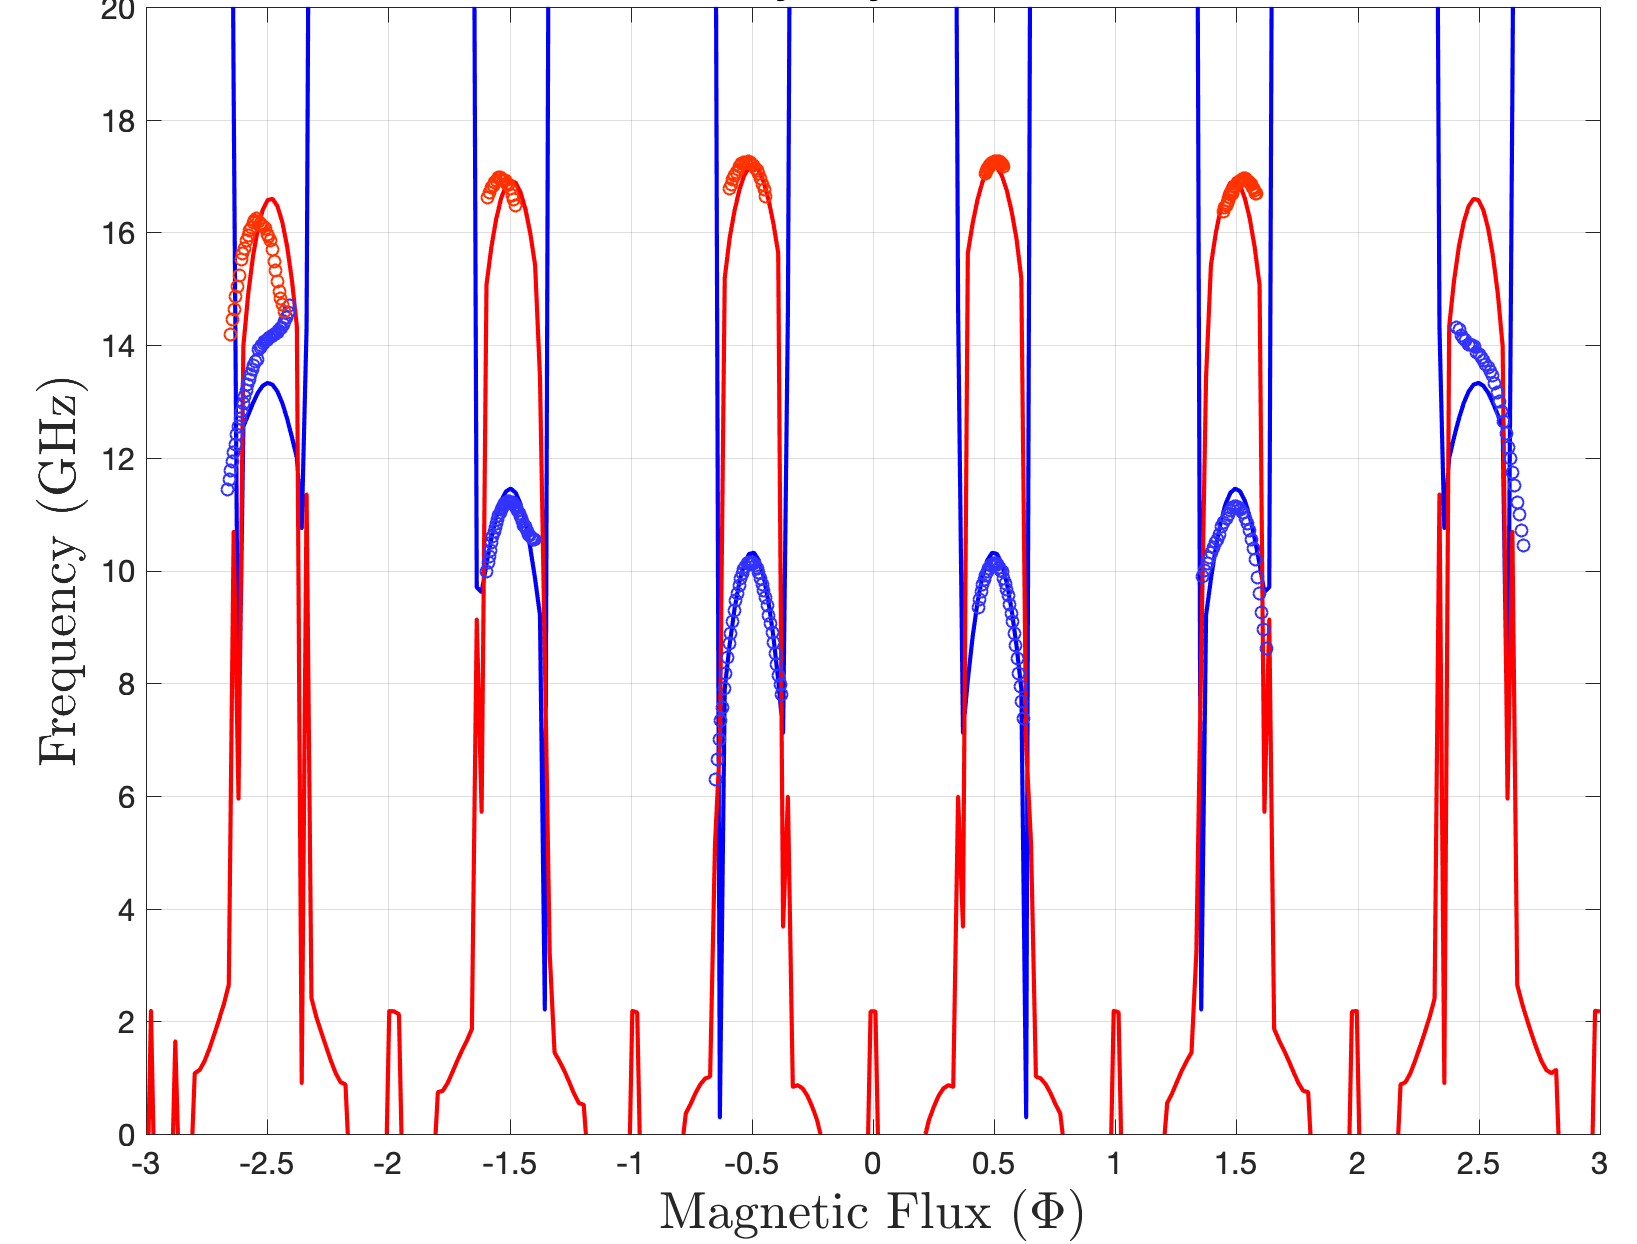
\includegraphics[height = 6cm]{figure3_qubit2}
 	\caption{Experimental results were fitted with $ E_J = \iunit{91}{GHz}, E_C = \iunit{13.5}{GHz}, \alpha = \iunit{1.023}{} $, (compared to \iunit{E_C = 10}{GHz}, \iunit{E_J=16}{GHz}, \iunit{\alpha = 1.05}{} expected from fabrication) and an assymetry between the areas of the loops of $ 1.011 $ was introduced. Asymmetry was introduced in order to increase the transition energies away from the turning point. \label{fig:simulation}}
 \end{figure}

\section{Dipole transition and relaxation}
 The flatness of the energy bands at the turning points, ensure weak sensitivity of the transition energies to flux fluctuations, and therfore the coherence of the qubit operation should be enhanced, compare to other flux qubits. We extract the decoherence time from Rabi oscillations, see Fig.~\ref{fig:rabi}, $ T_2 = \iunit{42}{ns} $ which is high for a qubit fabricated on standard technology. \includeref{the $ T_2 = \iunit{250}{ns} $ demonstrated by other qubits} 

 \begin{figure}[h!]
 	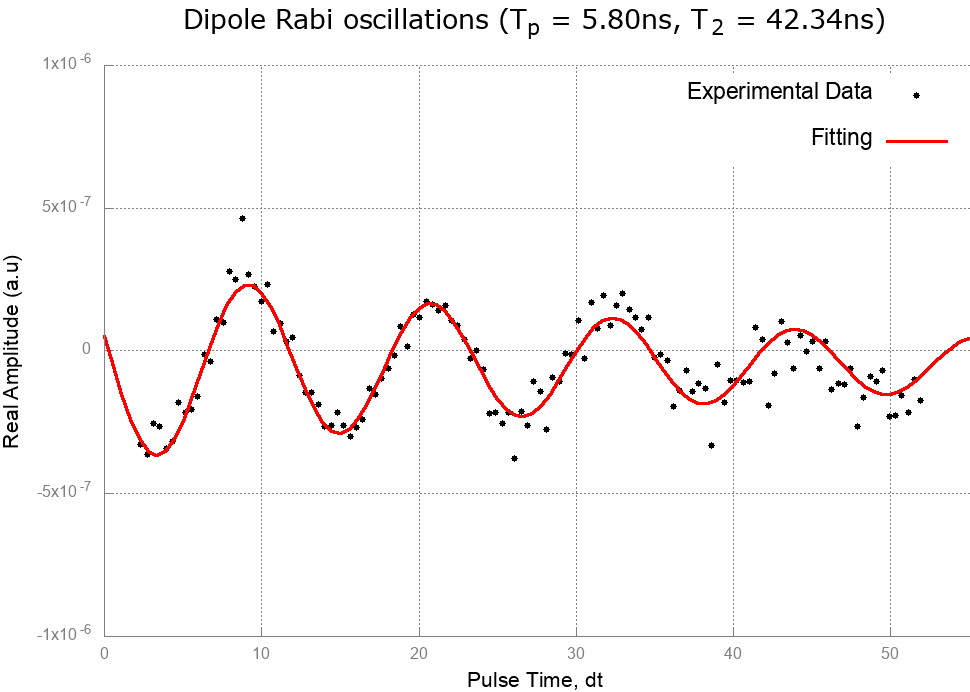
\includegraphics[height = 6cm]{figure5}
 	\caption{The qubit demonstrated a decoherence time $ T_2 = \iunit{42}{ns} $ from Rabi oscillation measurements. \label{fig:rabi}}
 \end{figure}

 \noindent We calculate the frequency $ \Gamma_{21} $ associeted with the dipole transition between eigenstates \iket{1} and \iket{2}, by evaluating the matrix element $ \bra{2}T\iket{1} $

 
	\begin{equation}\label{key}
	\Gamma_{21} = \hbar\omega_{21}\frac{\iabsSquared{\bra{2}T\iket{1}}}{\hbar^2Z_0}.
	\end{equation}
 
 \noindent The regions of a resonant transmission spectrum, with a large $ \Gamma_{21} $, cluster around the turning points $ \Phi = (n+\frac{1}{2})\Phi_0, n\in\mathcal{Z} $, see Fig.~\ref{fig:dipole_transition}. The qubit has the strongest coupling between states \iket{1} and \iket{2}, and therefore they are ideal for state operations with an external driving field.
 \begin{figure}
	\centering
 		\includegraphics[height=6.5cm]{figure4_v1}
 	\caption{The dipole transition rate $ \Gamma $ is proportional to the dipole transition element $ \bra{2}T\ket{1} $, where $ T $ is the charge operator responsible for the transition, and $ \iket{1} $ and \iket{2} are the eigenstates of the system. %There is strong transition between the levels at the turning point in magnetic flux, $ \Phi = (n+\frac{1}{2})\Phi_0, n\in\mathcal{Z} $.
 		\label{fig:dipole_transition}}
 \end{figure}
